
\documentclass[12pt]{beamer}

\usepackage[white]{beamerthemeWisconsin}
\usepackage{framed}
\usepackage{float}
\usepackage{booktabs}
\usepackage{tikz}
\usepackage{hyperref}
\usepackage{adjustbox}

%\usetheme[white]{Wisconsin}
\graphicspath{{./}{./uw-beamer-template/}{../images/}}
\title{Leveraging Intel's Embree Ray Tracing in the DAGMC Toolkit}
\author{Patrick C. Shriwise}
\institute{University of Wisconsin - Madison}
\date{ANS Winter Meeting 2015}




\AtBeginSection[]{
  \begin{frame}
  \vfill
  \centering
  \begin{beamercolorbox}[sep=8pt,center,shadow=true,rounded=true]{title}
    \usebeamerfont{title}\insertsectionhead\par%
  \end{beamercolorbox}
  \vfill
  \end{frame}
}


%%%% TIKZ OBJECTS %%%%
\usetikzlibrary{shapes}
\usetikzlibrary{positioning}
\usetikzlibrary{decorations.pathreplacing}
\usetikzlibrary{calc}

\tikzset{every node/.style={inner sep=0pt, outer sep=1pt}}
\tikzstyle{uwstep} = [minimum width=2.5cm, minimum height=1cm,text centered, text width=2.5cm, draw=black, fill=UWRed, text=white]

\tikzstyle{mbelement} = [rectangle, minimum width=0.5cm, text centered, text width=0.5cm, draw=black, fill=blue, text=white, inner sep=1pt, outer sep=0pt]

\tikzstyle{embreestep} = [ellipse, minimum width=2.5cm, minimum height=1cm,text centered, text width=2cm, draw=black, fill=blue, text=white, outer sep=0pt]

\tikzstyle{arrow} = [thick,->,>=stealth]

\tikzset{
    myarrow/.style={
        draw,
        fill=UWRed,
        single arrow,
        minimum height=4ex,
        single arrow head extend=1ex
    }
}

\newcommand{\arrowup}{%
\tikz [baseline=-0.5ex]{\node [myarrow,rotate=90] {};}
}
\newcommand{\arrowdown}{%
\tikz [baseline=-1ex]{\node [myarrow,rotate=-90] {};}
}
\newcommand{\arrowright}{%
\tikz [baseline=-0.5ex]{\node [myarrow,rotate=0] {};}
}
\newcommand{\doublearrow}{%
\tikz [baseline=-1ex]{\node [mydoublearrow,rotate=0] {};}
}



%%%% START DOCUMENT %%%%
\begin{document}


%% Title Frame %%
\frame{\titlepage \addtocounter{framenumber}{-1}}


%%Outline%%
%% \begin{frame}
%% \frametitle{Content}
%% \tableofcontents
%% \end{frame}

%% Introduction %%
\section{CAD-Based Monte Carlo Transport} % 1-2 slides
% We use it for our geometric queries:
   % point-inclusion
   % dist to next surf
% Replaces analytic intersections in native MonteCarlo packages
% Motivation: takes too long!
% Images of typical production models?
\begin{frame}

\frametitle{Robust CAD-Based Monte Carlo Transport}

DAGMC can robustly do transport calculations on detailed CAD models like these:


\begin{center}
\begin{tabular}{c c}

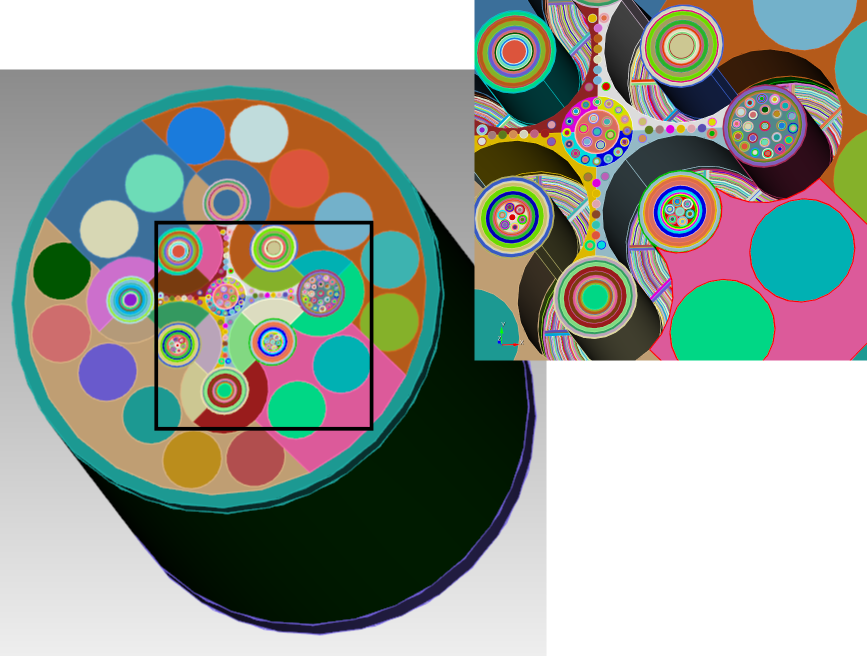
\includegraphics[height=0.4\textheight]{atr_both.png} &
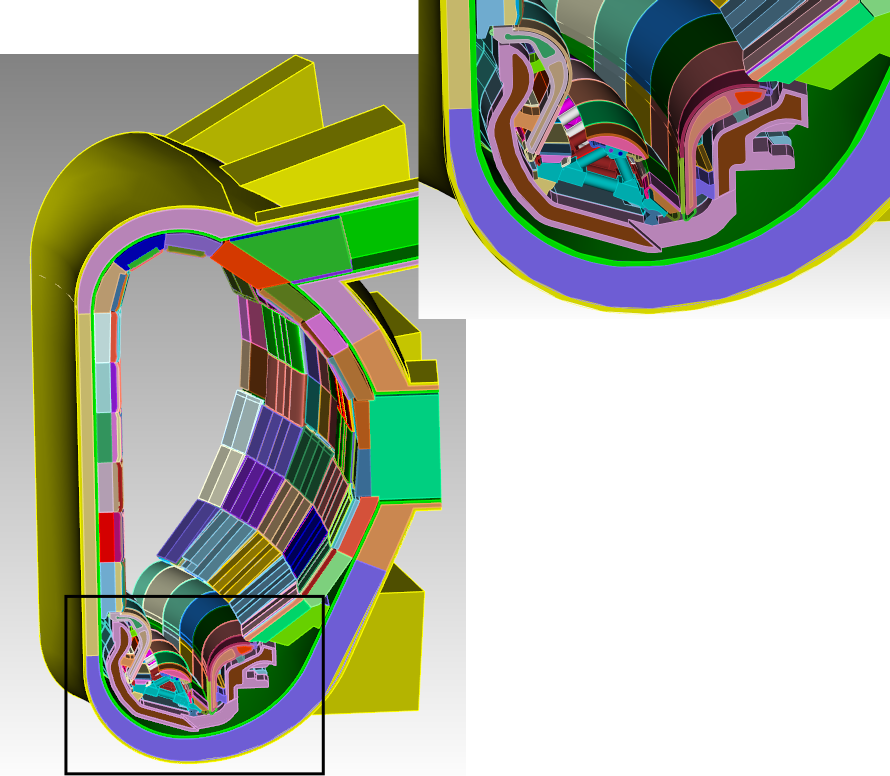
\includegraphics[height=0.4\textheight]{bllite_both.png} \\

\small Advanced Test Reactor &
\small ITER \\

\end{tabular}
\end{center}

But it takes a long time... (2-10x slower than native codes)

\end{frame}

\begin{frame}
\frametitle{DAGMC Workflow}
\begin{center}
  \begin{tikzpicture}
    \node (CAD) [uwstep] {\small CAD};
    
    \pause %%%%
    \visible<2>{\node (CAD L) [auto,outer sep=0pt,below = 0.1 cm of CAD] {\small geometric design};
      \node (fng cad)[auto,below = 0.1cm of CAD L,outer sep=0pt] {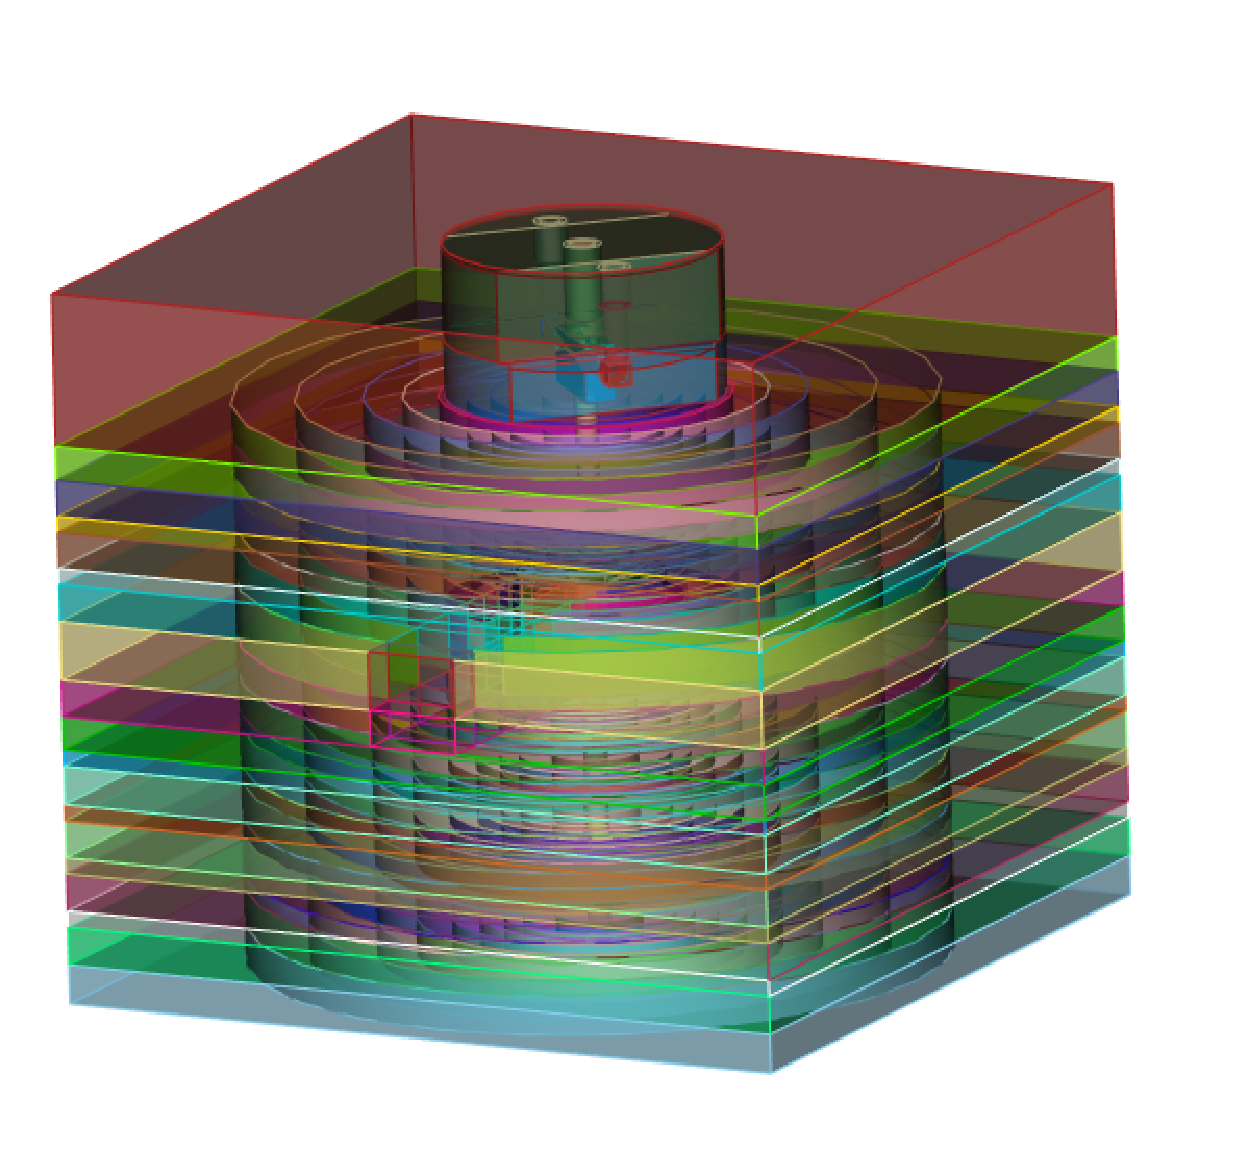
\includegraphics[scale=0.07]{fng_cad.png}};
      \node [auto,below = 0.1cm of fng cad, outer sep = 0 pt] {FNG};
    }
    
    \pause %%%%
    \node (PREPROC) [uwstep, right = 0.5cm of CAD] {\small preprocessing};
    \draw [arrow] (CAD) -- (PREPROC);
    
    \pause %%%%
    \visible<4>{\node (PREPROC LA) [auto,outer sep=0pt,above = 0.1cm of PREPROC] {\small surface faceting};
      \node (PREPROC LB) [auto,outer sep=0pt,below = 0.1cm of PREPROC] {\small facet sealing};
      \node [auto,below = 0.1cm of PREPROC LB,outer sep=0pt] {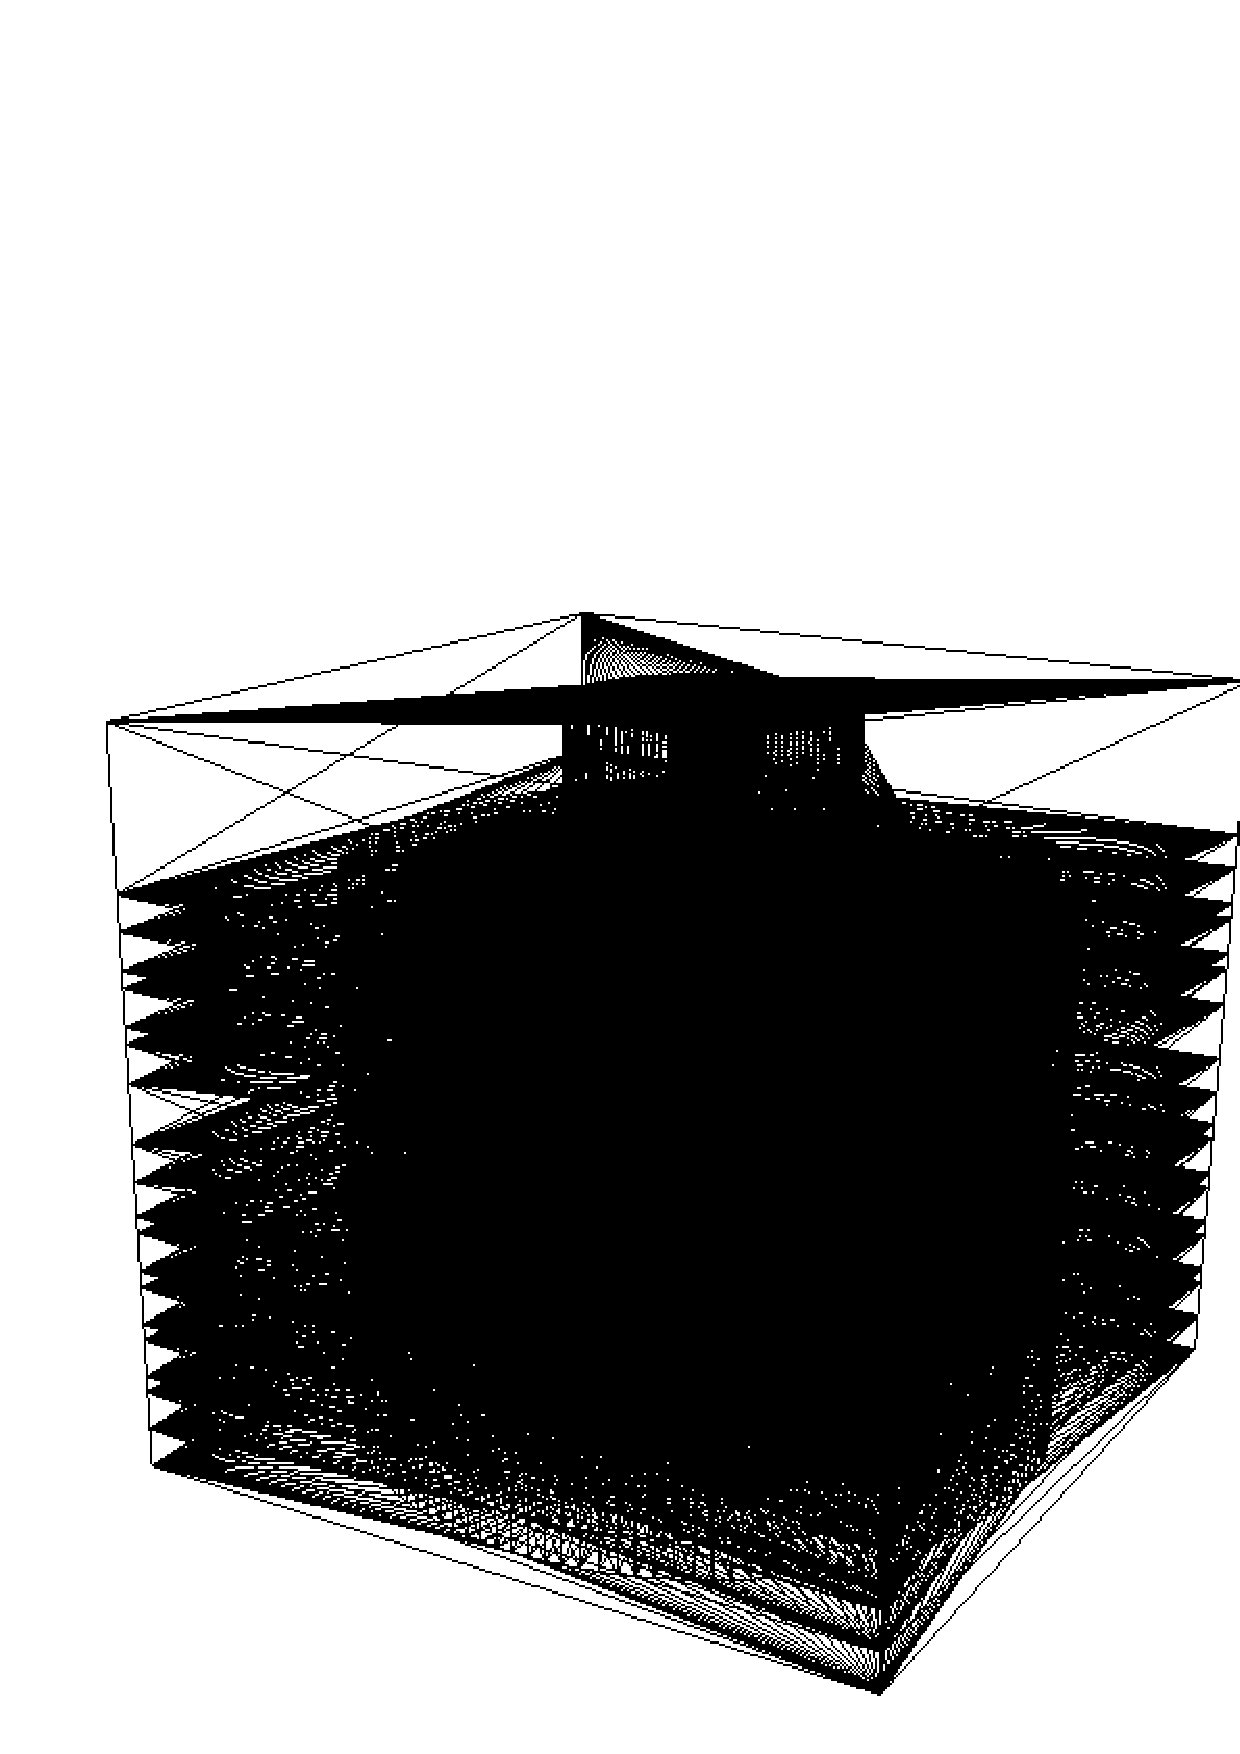
\includegraphics[scale=0.07]{fng_facets.png}};
    \node[auto,above= 0.3cm of PREPROC LA,outer sep=0pt] {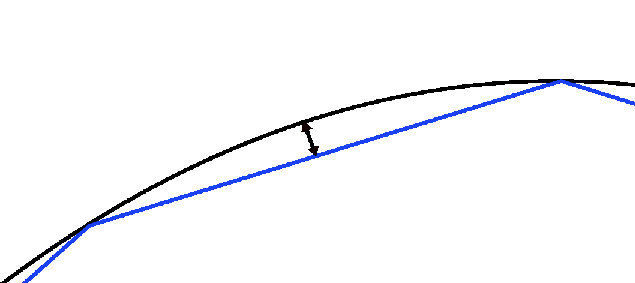
\includegraphics[scale=0.1]{facet_tol_zoomed.png}};}
    
    \pause %%%%
    \node (DAGMC) [uwstep, right = 0.5 cm of PREPROC] {\small DAGMC};
    \draw [arrow] (PREPROC) -- (DAGMC);
    
    \pause %%%%
    \node (MC) [uwstep, right = 0.5cm of DAGMC] {\small Monte Carlo};
    \draw[-latex] (DAGMC) to[bend right=10] node[above,rotate=60] {} (MC);
    \draw[-latex] (MC) to[bend right=10] node[above,rotate=60] {} (DAGMC);

    \pause %%%%
    \visible<7->{\node [auto,above = 0.6cm of MC,xshift=-1.5cm,outer sep=0pt] {Analysis Toolkit};}
    \draw [black,dotted] ($(DAGMC.north west)+(-0.15,0.5)$) rectangle ($(MC.south east)+(0.15,-0.5)$); 
    \pause %%%%
    \visible<8->{\node (MC LB) [auto,below = 0.1cm of MC, outer sep=0pt] {\small physics};}

    \pause %%%%
    \visible<9->{\node (DAGMC LA) [auto, above = 0.1cm of DAGMC, outer sep=0pt] {\small geometric queries};
    \node (DAGMC LB) [auto, below = 0.1cm of DAGMC, outer sep=0pt] {\small ray tracing};}

    \pause %%%%
    \visible<10>{\node (MC LA) [auto, above = 0.1cm of MC, outer sep=0pt] {\small Fluka};}

    \pause %%%%
    \visible<11>{\node (MC LA) [auto, above = 0.1cm of MC, outer sep=0pt] {\small Geant4};}

    \pause %%%%
    \visible<12>{\node (MC LA) [auto, above = 0.1cm of MC, outer sep=0pt] {\small ...};}

    \pause %%%%
    \visible<13>{\node (MC LA) [auto, above = 0.1cm of MC, outer sep=0pt] {\small MCNP5};}

    \pause %%%%
    \node (TOOLKIT L) [auto,below = 0.6cm of MC,xshift=-1.5cm,outer sep=0pt] {DAGMCNP};

    \pause %%%%
    \node [auto,below = 0.1cm of TOOLKIT L,outer sep=0pt] {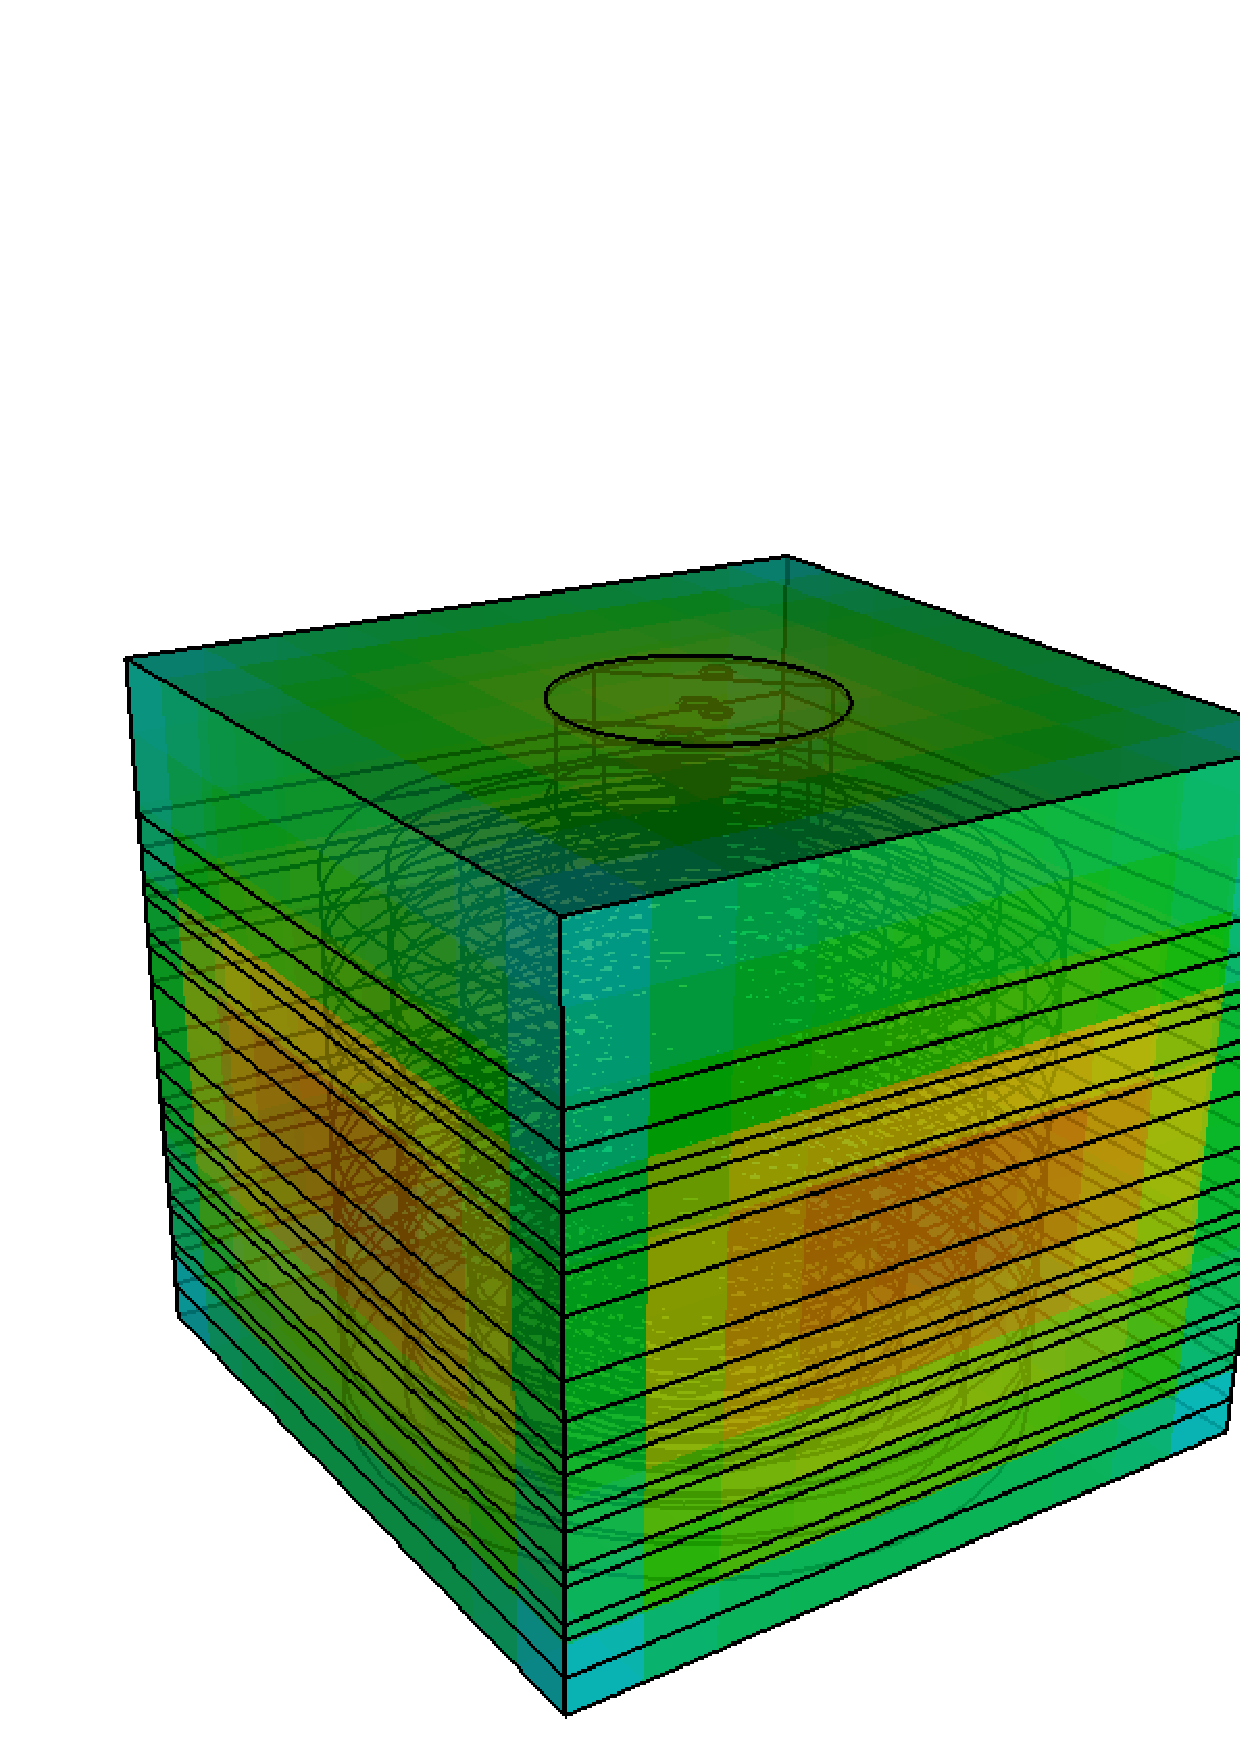
\includegraphics[scale=0.07]{fng_results.png}};
    
    \onslide<1->
  \end{tikzpicture}
\end{center}

\end{frame}

\begin{frame}

\frametitle{Ray Tracing in DAGMC}
 85\% of the time spent in DAGMC runs is in ray tracing of the discretized (faceted) model.

\begin{itemize}
\item point-inclusion tests
\item next surface distance determination
\item nearest surface to location
\end{itemize}



\end{frame}

\begin{frame}

  \frametitle{DAGMC \& Ray Tracing}
  
  A great deal of \textbf{human time} is saved in dealing with text-based geometric representations, but it comes at the cost of additional \textbf{computing time}.
 \vfill
 What if we can drastically reduce this extra computing time?

 \vfill

  
\end{frame}

\begin{frame}
  \frametitle{Embree}
  \begin{center}
    \begin{tikzpicture}
    \node (room) [auto] {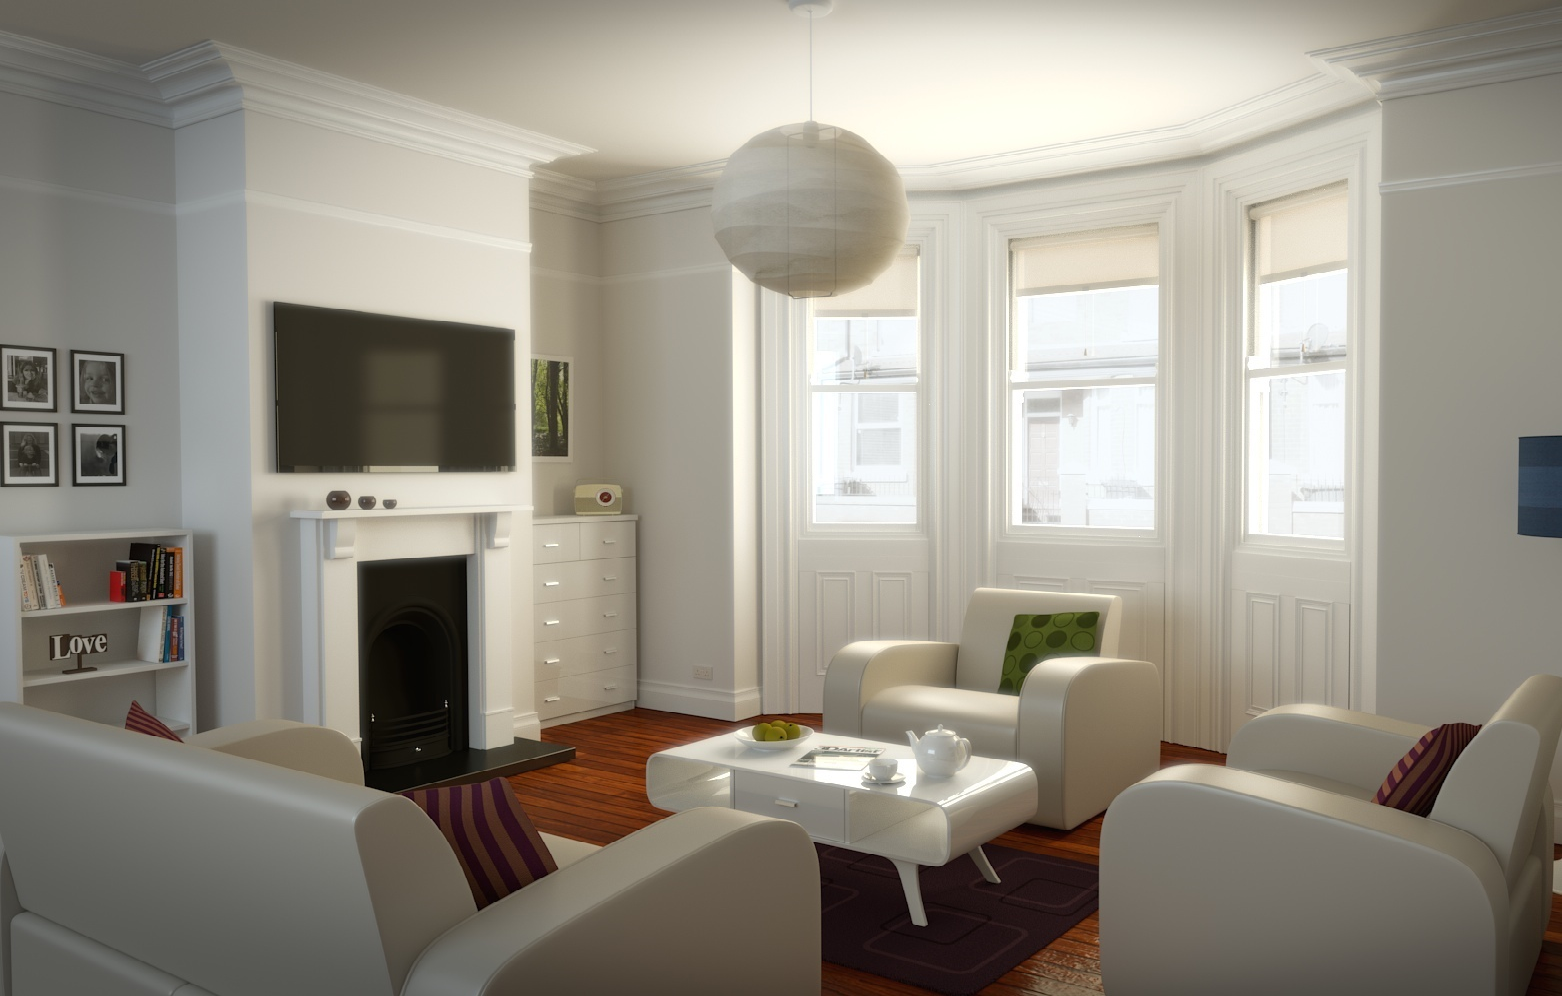
\includegraphics[width=0.28\textwidth]{2014-Siggraph-Embree-000.png}};
    \node (crown) [auto,right = 0.1cm of room] {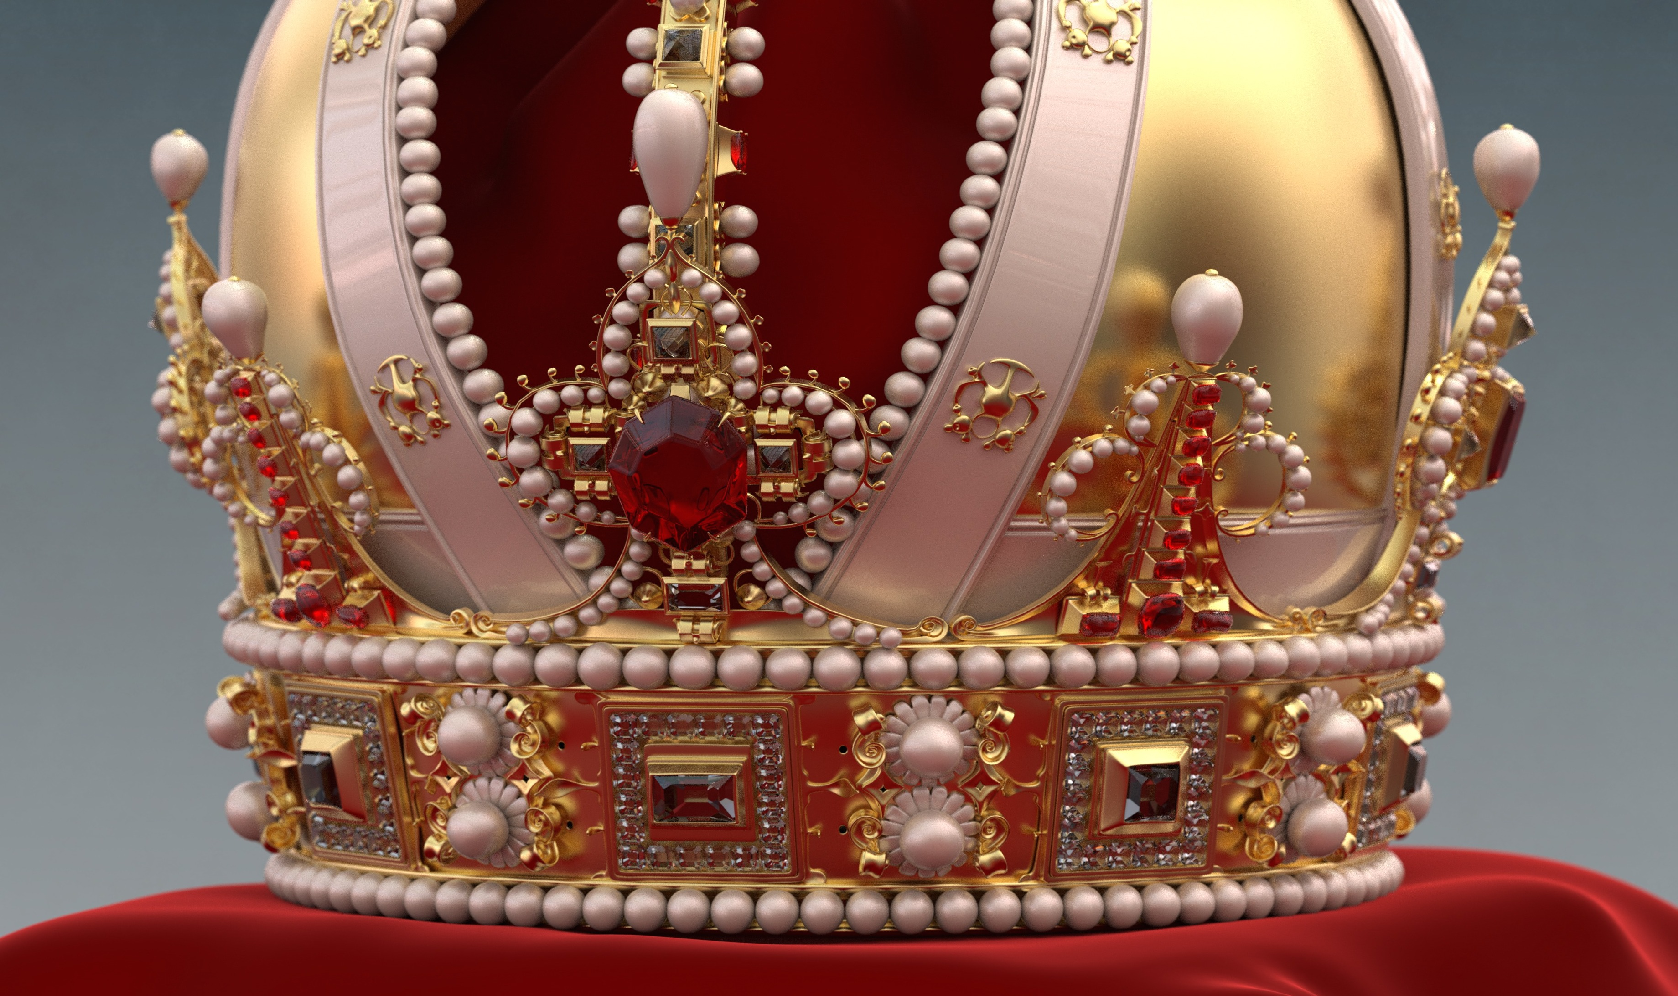
\includegraphics[width=0.3\textwidth]{2014-Siggraph-Embree-003.png}};
    \node (wayback) [auto,right = 0.1cm of crown] {
\includegraphics[width=0.31\textwidth]{2014-Siggraph-Embree-002.png}};
  \end{tikzpicture}
  \end{center}
  A high performance ray tracing kernel. \cite{embree}
  \vfill
  \begin{itemize}
  \item open source CPU-based project developed by Intel
  \item intended application is rendering
  \item successfully used in several commercial rendering packages
  \end{itemize}

  
\end{frame}


\section{Accelerating Ray Tracing} % 2-3 slides
% BVH explanation in 1 slide
% Embree's tricks
% Extra: SAH


\begin{frame}
\frametitle{Bounding Volume Hierarchies}


By partitioning the geometry-based meshes using bounding entities, we gain significant improvements over a linear search of the discrete elements.
\begin{columns}
  \column{0.5\textwidth}
  \begin{figure}
    \centering
    \begin{flushleft}\cite{gottschalk1996obbtree}\end{flushleft}
    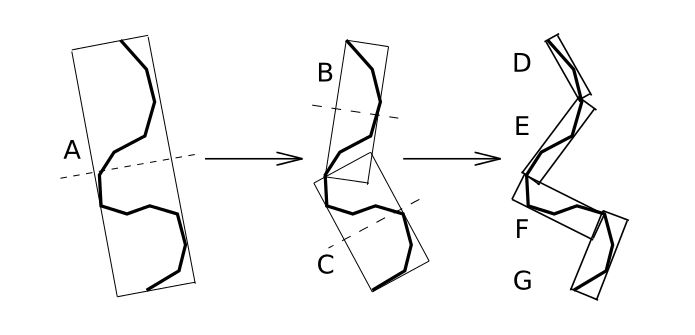
\includegraphics[width=1.1\textwidth]{bvh_2d_ex_w_labels.png} 
  \end{figure}
  
  \column{0.4\textwidth}
  \begin{figure}
    \centering
    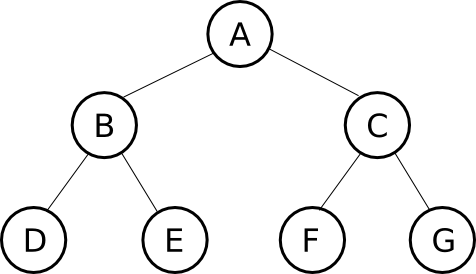
\includegraphics[width=0.7\textwidth]{binary_graph.png}
  \end{figure}
\end{columns}
\vfill
How these bounding volume hierarchies (BVHs) are created and traversed affects the performance \textbf{greatly}.


\end{frame}

\begin{frame}
\frametitle{DAGMC's BVH}

DAGMC uses the BVH hierarchy found in the Mesh Oriented dAtaBase, MOAB \cite{moab}.
\begin{center}
  \begin{tikzpicture}

    \node (SHALLOW) [auto, outer sep=10pt, label=below:{\small shallow}] {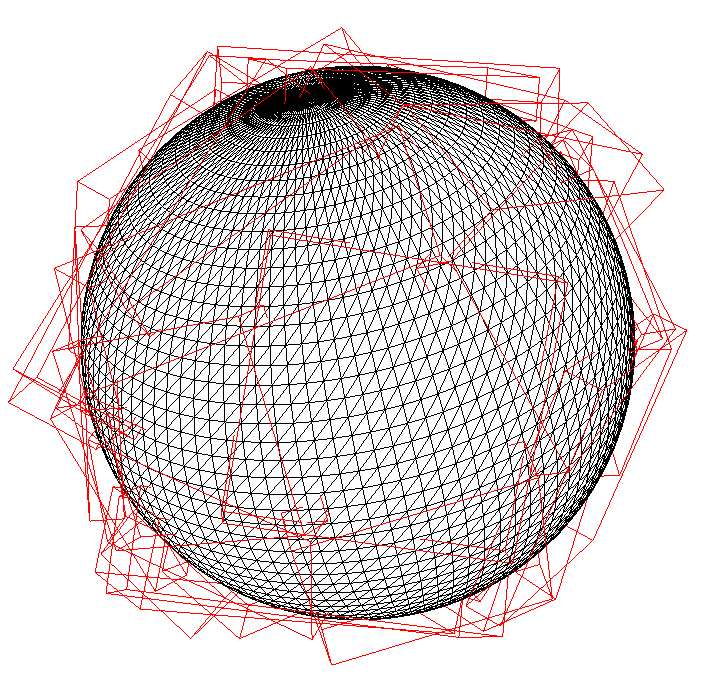
\includegraphics[width=0.3\textwidth]{sphere_obbs_shallow.png}};
    \node [myarrow,rotate=0,xshift=3.5cm] {};
    \node (DEEP) [auto, outer sep=10pt, xshift=7cm, label=below:{\small deep}] {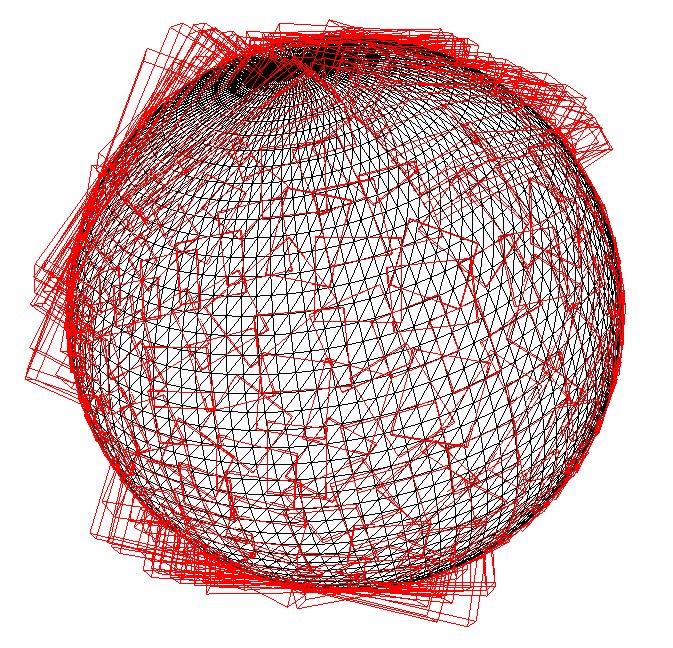
\includegraphics[width=0.3\textwidth]{sphere_obbs_deep.png}};

   % \draw [arrow] (SHALLOW) -- (DEEP);
  \end{tikzpicture}
\end{center}

\begin{itemize}
\item oriented bounding boxes (OBBs)
\item binary trees (as in prev. slide)
\item median splitting (longest to shortest axis)
\end{itemize}

\end{frame}



\begin{frame}

\frametitle{Embree's BVH}

Embree also uses OBBs but with a different tree structure:

\begin{center}
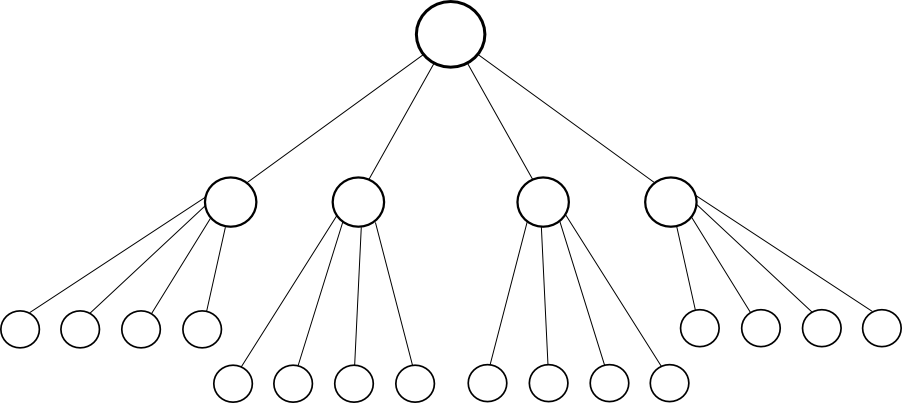
\includegraphics[width=0.5\textwidth]{quad_tree.png}
\end{center}

\begin{itemize}
\item median splitting w/ Surface Area Heuristic \cite{sah} criterion 
\item Quad-tree
  \begin{itemize}
  \item pro: discretizes the geometric primitives and space more finely per level in the tree
  \item con: makes for more tree nodes to check per query
  \end{itemize}
\item compensates by using advanced vector extensions (AVX) instruction sets to check many nodes at once.
\end{itemize}

\end{frame}


\section{Implementation of Embree in DAGMC} % 1-2 slides
% Maintaining watertightness
   % explain and refer to make_watertight
% Importance of the filter functions
   % allowed compliance with DAGMC conventions

\begin{frame}
  \frametitle{DAGMC entities in Embree}

  Embree has a limited capability for representing geometric topology, but enough to construct a mappable representation of DAGMC models.

\begin{center}
  \begin{tikzpicture}

    \node (VolA) [uwstep,text width=2cm] {\small DAGMC Volume};
    \node (SceneA) [embreestep, xshift=-3cm] {\small Embree Scene};

    \node (SurfA)[uwstep,xshift=3.5cm] {\small DAGMC Surface};
    \node (GeomA)[embreestep,xshift=6.5cm] {\small Embree Geometry};
    
    \node (SurfB) [uwstep,xshift=3.5cm,yshift=2cm,label={\small EntityHandle}] {\small DAGMC Surface};
    \node (GeomB) [embreestep,xshift=6.5cm,yshift=2cm,label={\small int id}] {\small Embree Geometry};

    \node (SurfC) [uwstep,xshift=3.5cm,yshift=-2cm] {\small DAGMC Surface};
    \node (GeomC) [embreestep,xshift=6.5cm,yshift=-2cm] {\small Embree Geometry};

    \draw[<->] (VolA) -- (SceneA);
    \draw[<->] (SurfA) -- (GeomA);
    \draw[<->] (SurfB) -- (GeomB);
    \draw[<->] (SurfC) -- (GeomC);
    \draw[->] (VolA) -- (SurfA);
    \draw[->] (VolA) -- (SurfB);
    \draw[->] (VolA) -- (SurfC);
  \end{tikzpicture}
  \end{center}

  
\end{frame}

\begin{frame}
\frametitle{make\_watertight}
\begin{itemize}
\item Applies faceted geometric information from CAD to remove topological ambiguity from the model \cite{make_watertight_smith_2010}
\end{itemize}
%%\vspace{-0.8cm}
\begin{center}
  \begin{tikzpicture}[scale=0.6, transform shape]
    \node (image) [yshift=-4cm] {\adjincludegraphics[scale=0.65,trim={ 20 80 0 90},clip]{sealing_ex.png}};
    \clip (current bounding box.south west) rectangle (current bounding box.north east);
    \pause
    %%%COPY1%%%
    \node (dot0) [yshift = -8cm,circle,xshift=-8cm,fill=blue,draw=black,minimum width=0.1cm] {};
    \node (dot1) at (dot0) [circle, fill=blue,xshift=1.3cm,yshift=0.6cm,draw=black,minimum width=0.1cm] {};
    \node (dot2) at (dot0) [circle, fill=blue,xshift=1.5cm,yshift=-0.75cm,draw=black,minimum width=0.1cm] {};
    \draw[-,color=orange] (dot0) -- (dot1);
    \draw[-,color=orange] (dot0) -- (dot2);
    \draw[-,color=orange] (dot2) -- (dot1);

    \node (cdot1) at (dot0) [circle, fill=blue,xshift=1.55cm,yshift=0.8cm,draw=black,minimum width=0.1cm] {};
    \node (cdot2) at (dot0) [circle, fill=blue,xshift=1.75cm,yshift=-0.55cm,draw=black,minimum width=0.1cm] {};
    
      \node (dot3) at (dot0) [circle, fill=blue,xshift=0cm,yshift=1cm,draw=black,minimum width=0.1cm] {};
      \draw [-,color=orange] (dot0) -- (dot3);
      \draw [-,color=orange] (dot1) -- (dot3);
      
      \node (cdot3) at (dot0) [circle, fill=blue,xshift=0.25cm,yshift=1.2cm,draw=black,minimum width=0.1cm] {};
      
      %%End surf A conn
      
      \node (dot4) at (dot0) [circle, fill=blue,xshift=1.75cm,yshift=1.95cm,draw=black,minimum width=0.1cm] {};
      \draw [-,color=black!60!green] (dot4) -- (cdot3);
      \draw [-,color=black!60!green] (dot4) -- (cdot1);
      \draw [-,color=black!60!green] (cdot3) -- (cdot1);
      
      
      \node (dot5) at (dot0) [circle, fill=blue,xshift=3cm,yshift=0.9cm,draw=black,minimum width=0.1cm] {};
      \draw [-,color=black!60!green] (dot5) -- (cdot1);
      \draw [-,color=black!60!green] (cdot2) -- (dot5);
      \draw [-,color=black!60!green] (cdot2) -- (cdot1);
      \draw [-,color=black!60!green] (dot4) -- (dot5);

      \pause
      %%%COPY2%%%
      \node (dot0) [below = -1.9cm of image,circle,right = of dot0, fill=blue,xshift=11cm,draw=black,minimum width=0.1cm] {};
      \node (dot1) at (dot0) [circle, fill=blue,xshift=1.3cm,yshift=0.6cm,draw=black,minimum width=0.1cm] {};
      \node (dot2) at (dot0) [circle, fill=blue,xshift=1.5cm,yshift=-0.75cm,draw=black,minimum width=0.1cm] {};
      \draw[-,color=orange] (dot0) -- (dot1);
      \draw[-,color=orange] (dot0) -- (dot2);
      \draw[-,color=orange] (dot2) -- (dot1);

     
      \node (dot3) at (dot0) [circle, fill=blue,xshift=0cm,yshift=1cm,draw=black,minimum width=0.1cm] {};
      \draw [-,color=orange] (dot0) -- (dot3);
      \draw [-,color=orange] (dot1) -- (dot3);
 

      %%End surf A conn
     
      \node (dot4) at (dot0) [circle, fill=blue,xshift=1.5cm,yshift=1.75cm,draw=black,minimum width=0.1cm] {};
      \draw [-,color=black!60!green] (dot4) -- (dot3);
      \draw [-,color=black!60!green] (dot4) -- (dot1);
      
      
      \node (dot5) at (dot0) [circle, fill=blue,xshift=2.75cm,yshift=0.7cm,draw=black,minimum width=0.1cm] {};
      \draw [-,color=black!60!green] (dot5) -- (dot1);
      \draw [-,color=black!60!green] (dot2) -- (dot5);

      \draw [-,color=black!60!green] (dot4) -- (dot5);
      \draw [-,color=red] (dot1) -- (dot3);
      \draw [-,color=red] (dot1) -- (dot2);
      \onslide<1->
      
    \end{tikzpicture}
\end{center}


\end{frame}




\begin{frame}
  \frametitle{Watertightness in EMDAG}
  Fortunately, we can maintain this topological watertightness in our Embree representation of the mesh.

  \begin{center}
    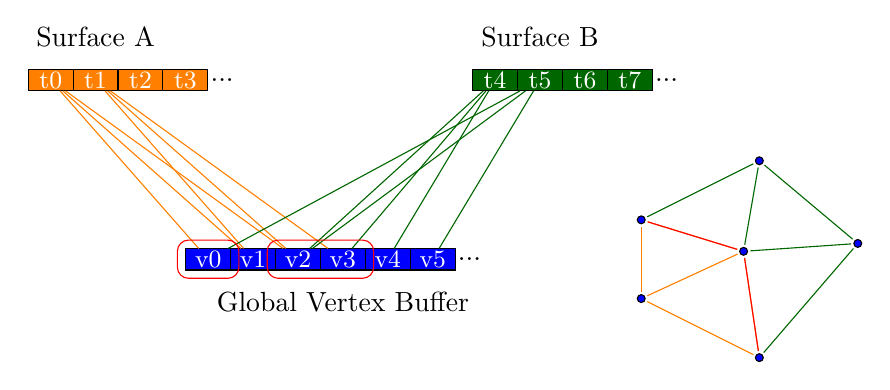
\begin{tikzpicture}

      %Vertices
      \node (v0) [mbelement] {\small v0};
      \node (v1) [mbelement, right = 0cm of v0] {\small v1};
      \node (v2) [mbelement, right = 0cm of v1] {\small v2}; 
      \node (v3) [mbelement, right = 0cm of v2] {\small v3}; 
      \node (v4) [mbelement, right = 0cm of v3] {\small v4}; 
      \node (v5) [mbelement, right = 0cm of v4] {\small v5}; 
      \node (ellipses) [auto,right = 0cm of v5] {...};
      \node (global vert buff) [auto, below = 0.25cm of v3] {Global Vertex Buffer};

      %Surface A
      \node (t0) [mbelement, fill=orange, above = 2cm of v0, xshift=-2cm] {\small t0};
      \node (t1) [mbelement, fill=orange, above = 2cm of v1, right = 0cm of t0] {\small t1};
      \node (t2) [mbelement, fill=orange, above = 2cm of v2, right = 0cm of t1] {\small t2};
      \node (t3) [mbelement, fill=orange, above = 2cm of v3, right = 0cm of t2] {\small t3};
%      \node (t4) [mbelement, fill=red, above = 2cm of v4, xshift=-3cm] {\small t4};
%      \node (t5) [mbelement, fill=red, above = 2cm of v5, xshift=-3cm] {\small t5};
      \node (ellipses) [auto,right = 0cm of t3] {...};
      \node (surfaceA) [auto,above = 0.25cm of t1] {Surface A};


      %Surface B
      \node (t4) [mbelement, fill=black!60!green, above = 2cm of v0, right = 3cm of ellipses] {\small t4};
      \node (t5) [mbelement, fill=black!60!green, above = 2cm of v1, right = 0cm of t4] {\small t5};
      \node (t6) [mbelement, fill=black!60!green, above = 2cm of v2, right = 0cm of t5] {\small t6};
      \node (t6) [mbelement, fill=black!60!green, above = 2cm of v3, right = 0cm of t6] {\small t7};
%      \node (t4) [mbelement, fill=red, above = 2cm of v4, xshift=-3cm] {\small t4};
%      \node (t5) [mbelement, fill=red, above = 2cm of v5, xshift=-3cm] {\small t5};
      \node (ellipses) [auto,right = 0cm of t6] {...};
      \node (surfaceB) [auto,above = 0.25cm of t5] {Surface B};
      
      \pause

      %ConnectivityTriangles
      \draw [-,color=orange] (t0) -- (v0);
      \draw [-,color=orange] (t0) -- (v1);
      \draw [-,color=orange] (t0) -- (v2);

      \node (dot0) [circle, fill=blue,xshift=5.5cm,yshift=-0.5cm,draw=black,minimum width=0.1cm] {};
      \node (dot1) at (dot0) [circle, fill=blue,xshift=1.3cm,yshift=0.6cm,draw=black,minimum width=0.1cm] {};
      \node (dot2) at (dot0) [circle, fill=blue,xshift=1.5cm,yshift=-0.75cm,draw=black,minimum width=0.1cm] {};
      \draw[-,color=orange] (dot0) -- (dot1);
      \draw[-,color=orange] (dot0) -- (dot2);
      \draw[-,color=orange] (dot2) -- (dot1);

      \pause

      \draw [-,color=orange] (t1) -- (v1);
      \draw [-,color=orange] (t1) -- (v2);
      \draw [-,color=orange] (t1) -- (v3);

      \node (dot3) at (dot0) [circle, fill=blue,xshift=0cm,yshift=1cm,draw=black,minimum width=0.1cm] {};
      \draw [-,color=orange] (dot0) -- (dot3);
      \draw [-,color=orange] (dot1) -- (dot3);
 

      %%End surf A conn
      \pause

      \draw [-,color=black!60!green] (t4) -- (v2);
      \draw [-,color=black!60!green] (t4) -- (v3);
      \draw [-,color=black!60!green] (t4) -- (v4);

      \node (dot4) at (dot0) [circle, fill=blue,xshift=1.5cm,yshift=1.75cm,draw=black,minimum width=0.1cm] {};
      \draw [-,color=black!60!green] (dot4) -- (dot3);
      \draw [-,color=black!60!green] (dot4) -- (dot1);
      
      \pause
      
      \draw [-,color=black!60!green] (t5) -- (v0);
      \draw [-,color=black!60!green] (t5) -- (v2);
      \draw [-,color=black!60!green] (t5) -- (v5);

      \node (dot5) at (dot0) [circle, fill=blue,xshift=2.75cm,yshift=0.7cm,draw=black,minimum width=0.1cm] {};
      \draw [-,color=black!60!green] (dot5) -- (dot1);
      \draw [-,color=black!60!green] (dot2) -- (dot5);


      \pause
      \draw [-,color=black!60!green] (dot4) -- (dot5);
      \draw [-,color=red] (dot1) -- (dot3);
      \draw [-,color=red] (dot1) -- (dot2);
      
      \draw[rounded corners, color=red ]
      ([xshift=-3pt,yshift=3pt]v2.north west) -- 
      ([xshift=3pt,yshift=3pt]v3.north east) -- 
      ([xshift=3pt,yshift=-3pt]v3.south east) -- 
      ([xshift=-3pt,yshift=-3pt]v2.south west) -- cycle;

      \draw[rounded corners, color=red ]
      ([xshift=-3pt,yshift=3pt]v0.north west) -- 
      ([xshift=3pt,yshift=3pt]v0.north east) -- 
      ([xshift=3pt,yshift=-3pt]v0.south east) -- 
      ([xshift=-3pt,yshift=-3pt]v0.south west) -- cycle;


    %% \nod2[circle,fill=none,minimum width=1cm,text width=6cm,draw=black,label={Global Vertex Buffer}] {};
    %% \draw plot [only marks, mark=*, mark size=0.5, domain=0:2.9, samples=250] (\x,{rand*sqrt(2.9^2-\x^2)});
    %% \begin{scope}[yscale=1,xscale=-1]
    %% \draw plot [only marks, mark=*, mark size=0.5, domain=0:2.9, samples=250] (\x,{rand*sqrt(2.9^2-\x^2)});
    %% \end{scope}

    %% \node[circle,outer sep=1pt,fill=none,minimum width=1cm,text width=3cm,draw=blue,xshift=1.5cm] (Surf1Circle) {};
    %% \node[auto,above=-0.6cm of Surf1Circle,fill=white] (Surf1) {\small \color{blue} Surface1};

    %% \node[circle,outer sep=1pt,fill=none,minimum width=1cm,text width=2cm,draw=red,yshift=-1cm] (Surf2Circle) {};
    %% \node[auto,above=-0.7cm of Surf2Circle,fill=white] (Surf2) {\small \color{red} Surface2};

    %% \node[circle,outer sep=1pt,fill=none,minimum width=3cm,text width=2cm,draw=green,xshift=-1cm,yshift=1cm] (Surf3Circle) {};
    %% \node[auto,above=-0.6cm of Surf3Circle,fill=white] (Surf3) {\small \color{green} Surface3};
    \onslide<1->
    \end{tikzpicture}
  \end{center}
  

\end{frame}

\section{Results} % 2-3 slides
% Pure ray fire comparison (no transport)
% Single volume tests
% Multiple volume tests

\begin{frame}
\frametitle{Ray Fire Test Models}

Rays were fired isotropically from the center of each of the following models:
\vfill

\begin{tikzpicture}
  \node (sphere) {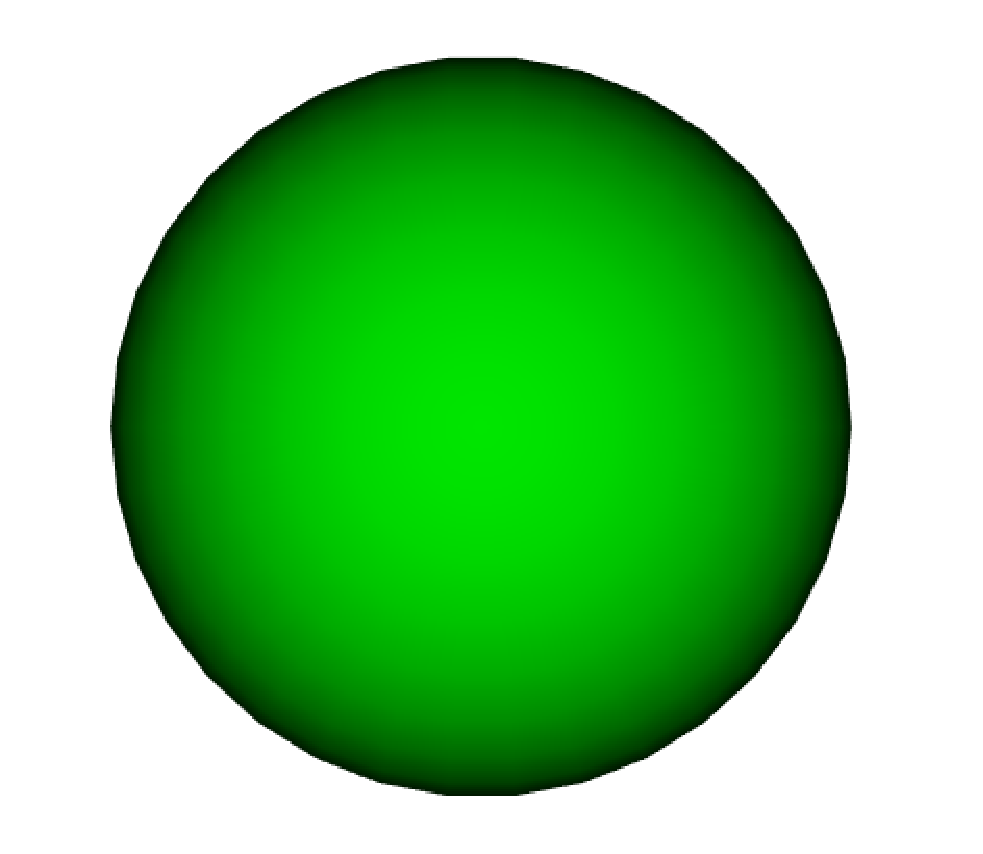
\includegraphics[scale=0.1]{sphere.png}};
  \node (ds) [right =  of sphere] {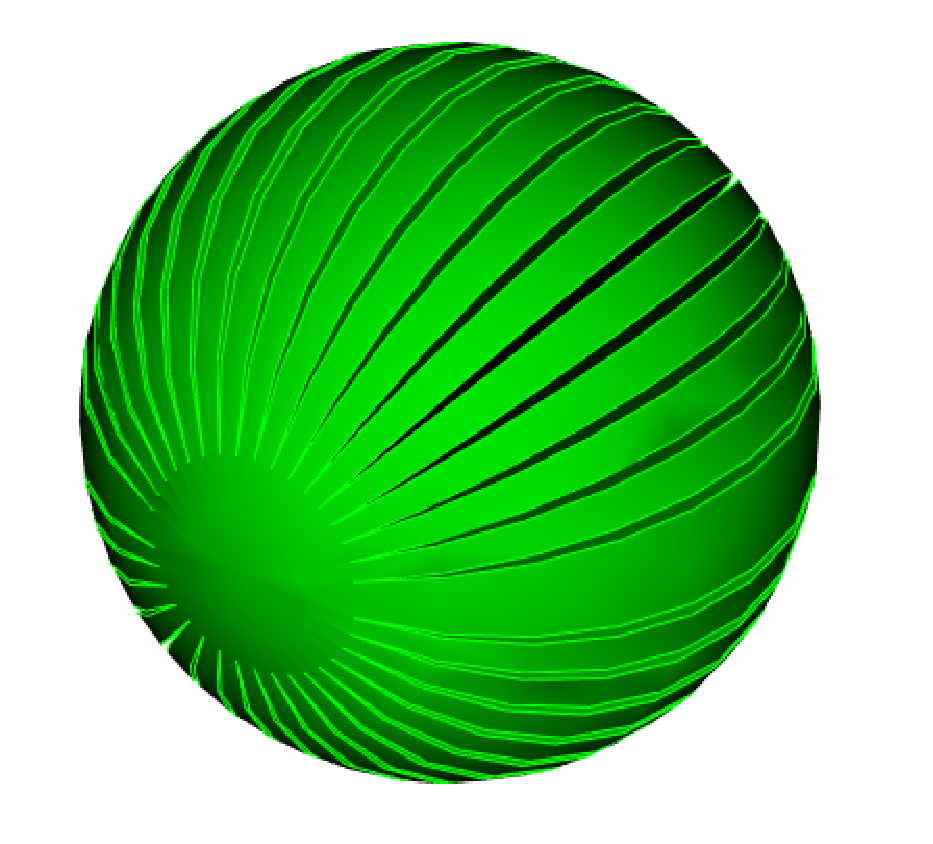
\includegraphics[scale=0.1]{ds.png}};
  \node (larcyl) [right =  of ds] {
\includegraphics[scale=0.1]{larcyl.png}};
  \pause 
  \node (sphere mesh) at (sphere.south east) [rotate=180,xshift=0.5cm] {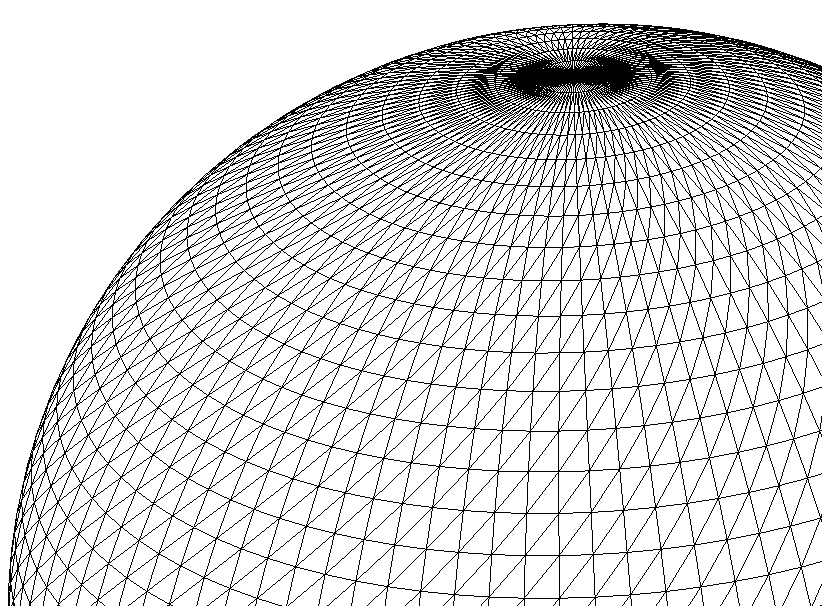
\includegraphics[scale=0.08]{sphere_mesh.png}};
  \pause
  \node (ds mesh) at (ds.north east) {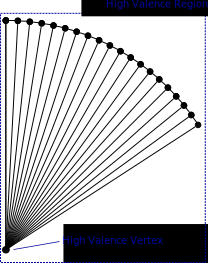
\includegraphics[scale=0.05]{hv.png}};
  \pause
  \node (lar cyl mesh) at (larcyl.south west) {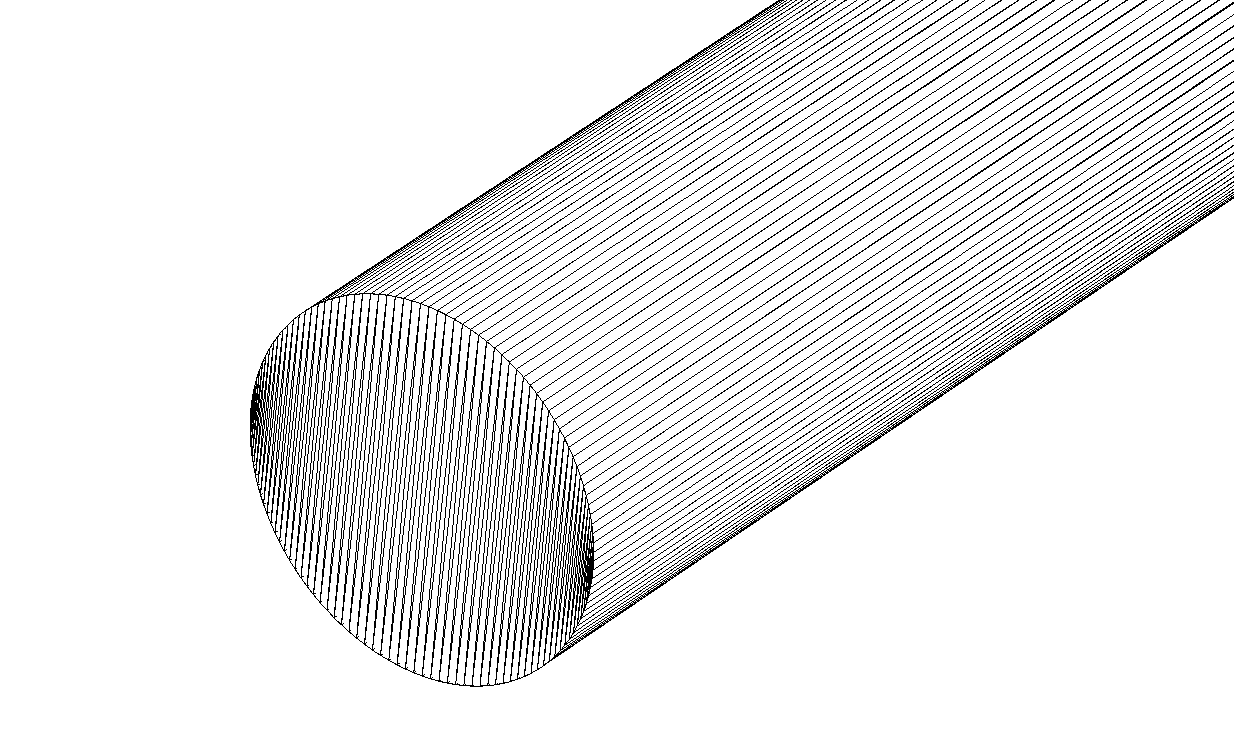
\includegraphics[scale=0.08]{lar_cyl_mesh.png}};
  \onslide<1->
\end{tikzpicture}


\end{frame}


\begin{frame}[c]
  \frametitle{Ray Fire Timings}
  \begin{center}
\begin{tikzpicture}
  \node (moab rf)  [auto,inner sep=0pt,inner sep=0pt,outer sep=0pt] {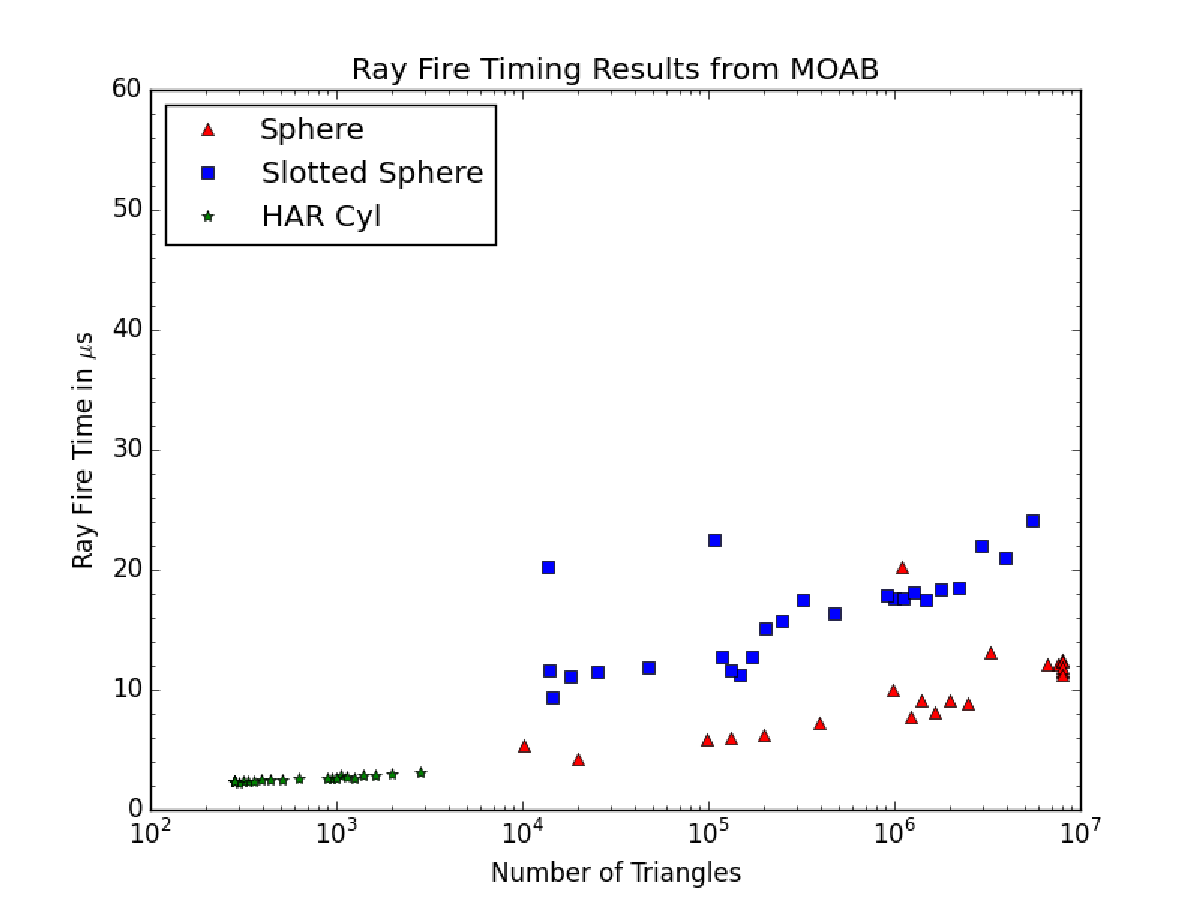
\includegraphics[trim={200 0 0 0 },scale=0.16]{Eig_fix_rf.png}};
  \node (emdag rf) [auto,right = -0.6cm of moab rf,inner sep=0pt,outer sep=0pt] {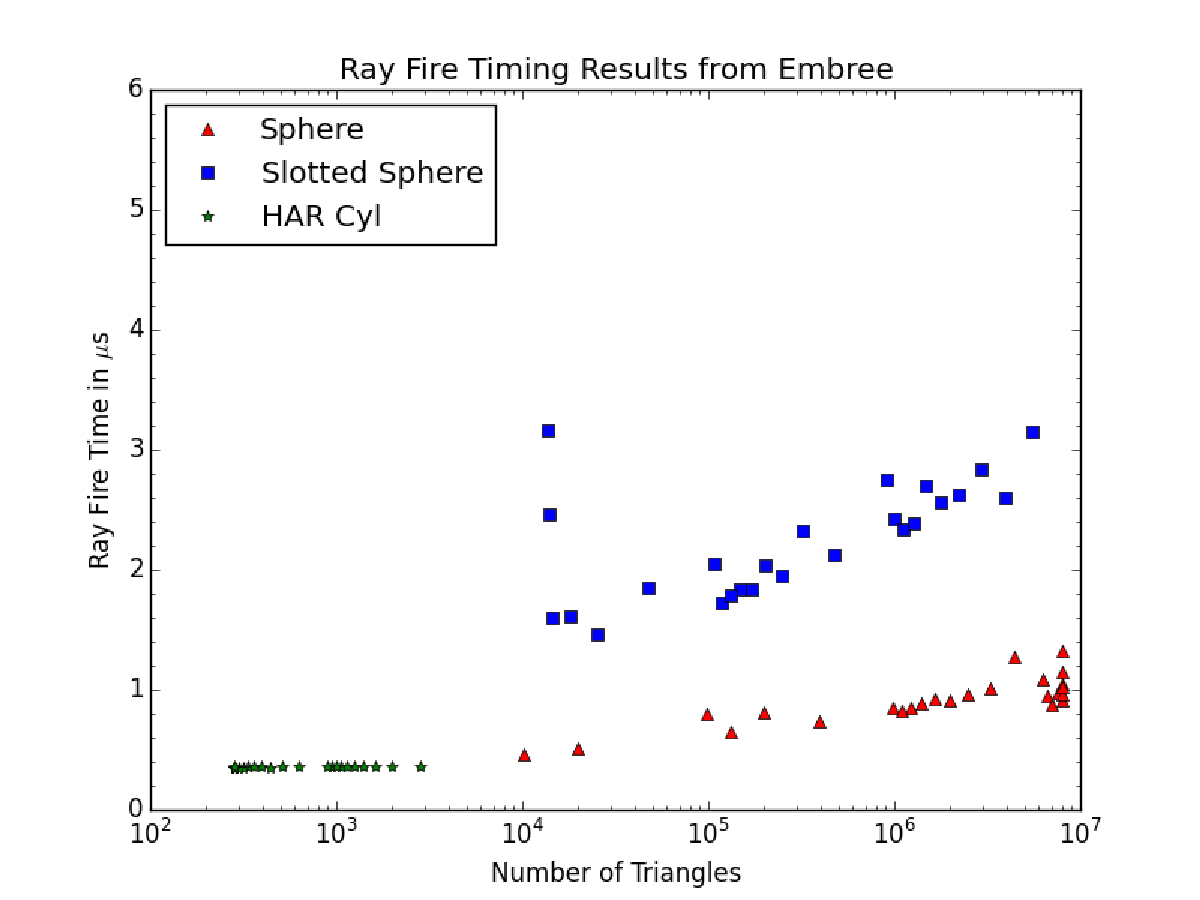
\includegraphics[scale=0.16]{embree_rf.png}};

  \node at (moab rf.north) [ellipse,draw=red,yshift=-0.5cm,xshift=-3.25cm,minimum width=0.5cm,minimum height=0.3cm] {};
  \node at (emdag rf.north) [ellipse,draw=red,yshift=-0.5cm,xshift=-2.6cm,minimum width=0.5cm,minimum height=0.3cm] {};
  \onslide<1->
\end{tikzpicture}
\end{center}
\begin{center}
  Embree was built using the AVX2 instruction set (not AVX) which allows more tree nodes to be visited in one command.
\end{center}

\end{frame}





\begin{frame}
\frametitle{Nested Volume Models}
\begin{itemize}
\item All were filled with non-physically dense hydrogen for a highly scattering medium. 
\item Isotropic point source of 5 MeV neutrons at the center.
\item 1M particle histories in each run.
\end{itemize}

\begin{center}
\begin{tikzpicture}

  \node (ns) [auto] {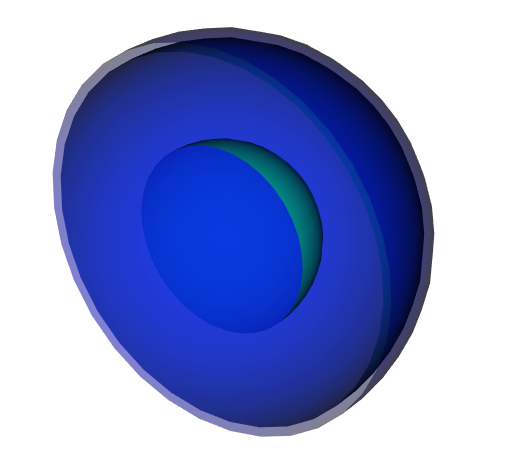
\includegraphics[scale=0.2]{nested_spheres.png}};
  \node (nc) [auto,right = of ns,xshift=0.25cm] {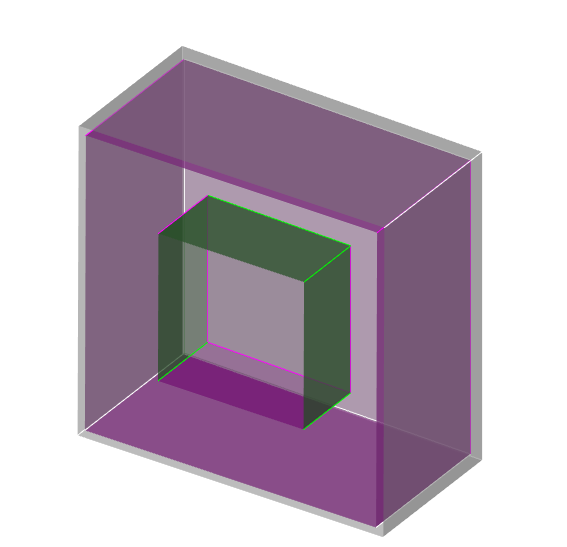
\includegraphics[scale=0.2]{nested_cubes.png}};
  \node (nsl) [auto,below = of ns] {Nested Spheres};
  \node [auto,right = of nsl,xshift=1.75cm] {Nested Cubes};

\end{tikzpicture}
\end{center}

\end{frame}


\begin{frame}
\frametitle{Nested Volume Results}

\begin{table}
  \small
  \begin{center}
    \label{nestedspheres}
    \begin{tabular}{lcccc}
      \toprule
      Value & MCNP5 & DAGMCNP & EMDAGMCNP \\
      \toprule
      %%Hist/min & 2.2991E+05 & 1.9877E+04 & 1.3947E+05 \\
      %%\hline
      \multicolumn{4}{l}{\textbf{Cell 1 Tallies}} \\
      \hline
      Flux  & 5.25725E-03 & 5.25734E-03 & 5.25734E-03 & ($cm^{-2}$) \\
      Energy  & 3.17869E-03 &  3.17873E-03 &  3.17873E-03 & (MeV/g) \\
      \hline
      \multicolumn{4}{l}{\textbf{Cell 2 Tallies}} \\
      \hline
      Flux  & 1.91645E-04 & 1.91644E-04 & 1.91644E-04 \\
      Energy  & 5.22131E-05 & 5.22137E-05 & 5.22137E-05 \\
      \hline
      \multicolumn{4}{l}{\textbf{Cell 3 Tallies}} \\
      \hline
      Flux  & 1.18371E-05 & 1.18{\color{red} 376}E-05 & 1.18{\color{red} 410}E-05 \\
      Energy  & 4.96282E-06 & 4.96285E-06 & 4.96285E-06 \\
      \bottomrule
                        
    \end{tabular}
    \vfill
    Zero lost particles \\
    Discrepancy caused by a single particle \\

    
  \end{center}
%%\vspace{-0.2cm}
\end{table}

\end{frame}

\begin{frame}
\frametitle{Run Time Results}

\begin{table}
  \small
  \begin{center}

      \label{timings}
    \begin{tabular}{lccc}


      \toprule
      Test Model & MCNP5 & DAGMCNP & EMDAGMCNP \\
      %%\hline
      & \phantom{a} & \multicolumn{2}{c}{\textbf{run time/native time}} \\
      \hline
      Sphere & 1 & 12.27 & 1.61 \\
      Cube & 1 & 1.85 & 1.15 \\
      Nested Spheres & 1 & 8.89 & 1.83 \\
      Nested Cubes & 1 & 1.79 & 0.92 \\
      %% Sphere & 2.93 & 25.13 & 4.73  \\
      %% Cube & 5.03 & 10.56  & 5.80 \\
      %% Nested Spheres & 4.35 & 50.82 & 7.94 \\
      %% Nested Cubes & 4.73 & 9.26 & 4.35 \\
      \hline
      &  \multicolumn{3}{c}{\textbf{histories/min}} \\
      \hline
      Sphere & 3.41E+05  & 3.99E+04  & 2.18E+05   \\
      Cube & 1.99E+05 & 9.47E+04 & 1.73E+05 \\
      Nested Spheres & 2.29E+05 & 1.99E+04 & 1.39E+05 \\
      Nested Cubes & 2.12E+05 & 1.08E+05 & 2.30E+05 \\
      \bottomrule

      %% \toprule
      %% Test Model & MCNP & DagMCNP & EmDagMCNP \\
      %% %%\hline
      %% & \multicolumn{3}{c}{\textbf{time (min)}} \\
      %% \hline
      %% Sphere & 2.93 & 25.13 & 4.73  \\
      %% Cube & 5.03 & 10.56  & 5.80 \\
      %% Nested Spheres & 4.35 & 50.82 & 7.94 \\
      %% Nested Cubes & 4.73 & 9.26 & 4.35 \\
      %% %%\hline
      %% &  \multicolumn{3}{c}{\textbf{histories/min}} \\
      %% \hline
      %% Sphere & 3.4104E+05  & 3.9944E+04  & 2.1810E+05   \\
      %% Cube & 1.9879E+05 & 9.4738E+04 & 1.7260E+05 \\
      %% Nested Spheres & 2.2991E+05 & 1.9877E+04 & 1.3947E+05 \\
      %% Nested Cubes & 2.1170E+05 & 1.0806E+05 & 2.3026E+05 \\
      %% \bottomrule
      
    \end{tabular}
  \end{center}
\end{table}


\end{frame}

\begin{frame}
\frametitle{Limitations}

This was a nice proof of principle project for faster CAD-based analysis, but... \\
\vfill
\begin{itemize}
\item Embree uses single floating point precision
\item Lost particles in complex geometries, most likely due to conversions double to float
\end{itemize}
\end{frame}
% Extra: slide with graphic of our specific problem

\section{Looking Forward} % 2 slides

\begin{frame}

\frametitle{Future Work}

\vfill
The application of ray tracing in Monte Carlo differs from that of rendering
  \begin{itemize}
    \item almost entirely incoherent rays
    \item number of ray queries to achieve desired result
    \item etc.
  \end{itemize}
\vfill
How should our ray tracing kernels be different? Should they be different at all?

% Proof of principle
% Likely to see improvements in our native system using variations of these techniques
% Point them to pyembree for a simple example of a 1-D Monte Carlo calculation in 3 regions
\end{frame}


\section{Conclusions}

\begin{frame}
  \frametitle{Acknowledgements}
  \begin{center}
    This work is supported by the Nuclear Regulatory Comission Graduate Fellowship.
    \end{center}
  \end{frame}

%QUESTIONS - 1 slide
\begin{frame}

\begin{center}
\vfill
\huge {Questions?} \\
\vfill
\normalsize email: shriwise@wisc.edu
\vfill
\end{center}
\normalsize
Some useful links:
\begin{itemize}
\item \href{https://embree.github.io/}{{\color{blue}embree}} (https://embree.github.io/)
\item \href{https://github.com/scopatz/pyembree}{{\color{blue}pyembree}} (https://github.com/scopatz/pyembree)
\end{itemize}

\end{frame}


\begin{frame}
\frametitle{Single Volume Results}

\begin{table}[h]

  \begin{center}

    \begin{tabular}{lccc}
     \toprule
      Value & MCNP & DAGMCNP & w/ EMDAGMCNP \\
     \toprule
     %%Hist/min & 1.9879E+05 & 9.4738E+04 & 1.7260E+05  \\
     %%\hline
     \multicolumn{4}{l}{\textbf{Flux} ($cm^{-2}$)} \\
     \hline
     Tally & 5.61374E-03 & 5.61374E-03 & 5.61374E-03 \\
     Err & 3E-4 & 3E-4 & 3E-4  \\
     FOM & 2.47008E+06 & 1.17719E+06 & 2.14469E+06 \\
     \hline
     \multicolumn{4}{l}{\textbf{Energy} (MeV/g)} \\
     \hline
     Tally & 2.98933E-03 & 2.98933E-03 & 2.98933E-03 \\
     Err & 7E-4 & 7E-4 & 7E-4 \\
     FOM & 3.99526E+05 & 1.90406E+05 & 3.46895E+05 \\
     \bottomrule
     
    \end{tabular}


  \end{center}
\vspace{-0.4cm}
\end{table}

\end{frame}



%Citations
\begin{frame}
  \bibliographystyle{ans}
  \footnotesize{\bibliography{bibliography}}
\end{frame}

\end{document}


